\documentclass[12pt]{article}
\usepackage{cite}
\usepackage{url}
\usepackage{graphicx}

\title{Harvest \\
\large subtrop: SA Subtropical Harvest Growers' Association
}
\author{Binary Ninjaz}

\date{}

\renewcommand{\and}{\\}

\begin{document}
	\begin{titlepage}
	
	\begin{center}
		% Upper part of the page         
        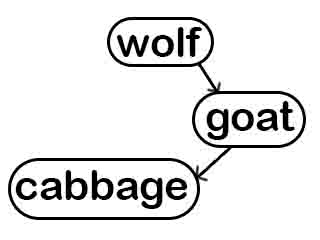
\includegraphics[width=0.7\linewidth]{team.jpg}\\[1cm]
		\textsc{\LARGE Binary Ninjaz}\\[0.3cm]
		% Title
		\rule{\linewidth}{0.5mm} \\[1cm]
		{ \huge \bfseries SUBTROP - Harvest 2018}\\[0.5cm]
		\rule{\linewidth}{0.5mm} \\[1cm] 		
  
		
		\begin{minipage}{0.4\textwidth}
			\begin{flushleft} \large
				\emph{} \\
				Sizo {Duma}
			\end{flushleft}
		\end{minipage}
		\begin{minipage}{0.4\textwidth}
			\begin{flushright} \large
				\emph{} \\
				15245579
			\end{flushright}
		\end{minipage}

		\begin{minipage}{0.4\textwidth}
			\begin{flushleft} \large
            	\emph{} \\
				John {Ojo}
			\end{flushleft}
		\end{minipage}
		\begin{minipage}{0.4\textwidth}
			\begin{flushright} \large
				\emph{} \\
				15096794 
			\end{flushright}
		\end{minipage}
		
		\begin{minipage}{0.4\textwidth}
			\begin{flushleft} \large
				\emph{} \\
				Kevin Reid
			\end{flushleft}
		\end{minipage}
		\begin{minipage}{0.4\textwidth}
			\begin{flushright} \large
				\emph{} \\
				15008739
			\end{flushright}
		\end{minipage}

		\begin{minipage}{0.4\textwidth}
			\begin{flushleft} \large
				\emph{} \\
				Shaun {Yates}
			\end{flushleft}
		\end{minipage}
		\begin{minipage}{0.4\textwidth}
			\begin{flushright} \large
				\emph{} \\
				16007493
			\end{flushright}
		\end{minipage}
        
        \begin{minipage}{0.4\textwidth}
			\begin{flushleft} \large
				\emph{} \\
				Letanyan {Arumugam}
			\end{flushleft}
		\end{minipage}
		\begin{minipage}{0.4\textwidth}
			\begin{flushright} \large
				\emph{} \\
				14228123 
			\end{flushright}
		\end{minipage}
		
		\begin{minipage}{0.4\textwidth}
			\begin{flushleft} \large
				\emph{} \\
				Teboho {Mokoena}
			\end{flushleft}
		\end{minipage}
		\begin{minipage}{0.4\textwidth}
			\begin{flushright} \large
				\emph{} \\
				14415888 
			\end{flushright}
		\end{minipage}
		\break
		\break
		
		\rule{\linewidth}{0.5mm} \\[1cm] 
		\textsc{\Large Stakeholders}\\[1cm]	
		
		\begin{minipage}{0.4\textwidth}
			\begin{flushleft} \large
				\emph{} \\
				subtrop: SA Subtropical Growers' Association
			\end{flushleft}
		\end{minipage}
		\begin{minipage}{0.4\textwidth}
			\begin{flushright} \large
				\emph{} \\
				Barry Christie
			\end{flushright}
		\end{minipage}

		
	\end{center}
\end{titlepage}
	
    \newpage
	\tableofcontents
	\newpage
	
	\section{Description}
	We envision using the mobile phones that the worker uses as simply a tracking device. They will not have to use it much other than to start a timer when they start working and stop it once their done. Their GPS location will be polled periodically. The final yield amount will then be entered at the end. The rest of the predictive analysis and summary data will then be appropriately calculated. The summary and predications can then be accessed on a summary screen. The summary screen can be displayed on the mobile application and on the web interface. The web interface will be a larger more customizable interface that will allow the farmers to do all their maintenance and administrative work. The farmers will then have full access to summaries, projection trends and real-time locations data of workers.
	
	The following diagram shows how we intend to structure the entire system. We also show what the main functions that each view will have to fulfil.
	
	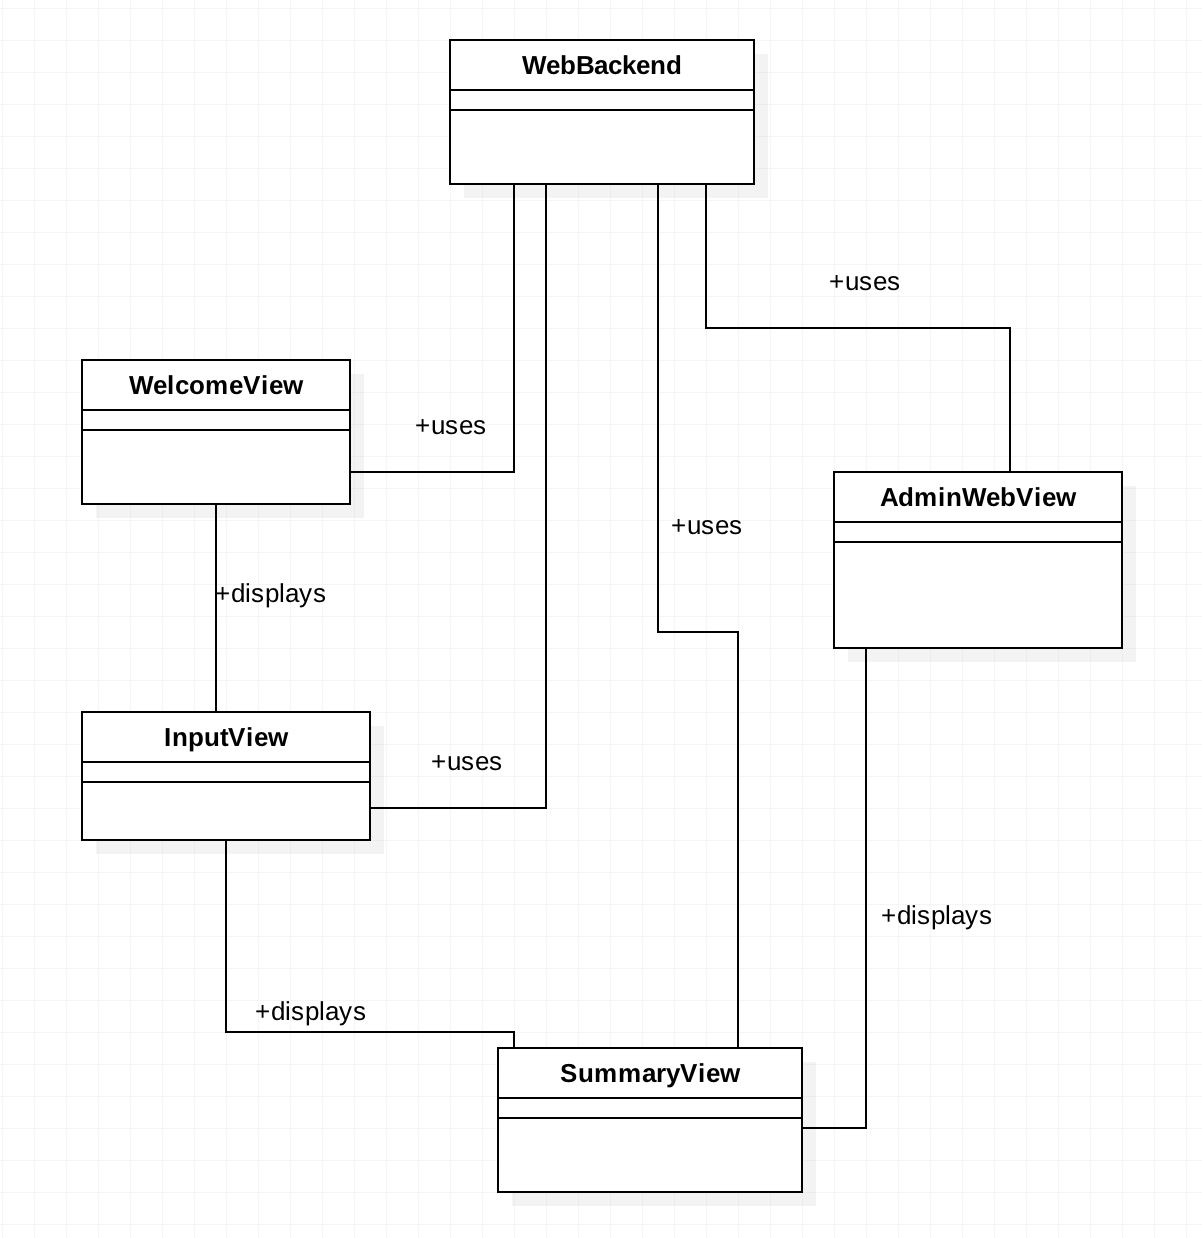
\includegraphics[scale=0.45]{Harvest.png}
	\newpage
	
	\section{Technologies We'll Use}
	\begin{enumerate}
	\item Languages: HTML, CSS, JavaScript, Java and Swift
	\item Geographic Data: Google Maps API
	\item IDE: Android Studio and XCode
	\item Persistent Storage: Firebase
	\item Version Control: Git/Github
	\end{enumerate}
	
	\section{Development Methodology}
	We will be using Github as a development/communication platform. Github is known for being able to serve massive, worldwide software projects. Using a great version/source control platform will allow us to implement an Agile software development method. We intend to combine all of our own unique development strategies in-order to build the best and most intuitive application possible. We believe that everything can be made easier. And we enjoying making it so! We see your problem as being perfectly catered towards having an elegant solution. Data capturing user interfaces were one of the very first problems people needed to solve, which means we have a lot of history and design principles to guide us towards an optimal solution. The hardest part of creating a great data capturing user experience is understanding the work flow of the capturers. To accomplish our goal we will require interviews with the participants using the application and interface. We believe this will allow us a true understanding, which will allow us to build the perfect system.
	
	\section{Who We Are}
	We are a capable collection of individuals with many varying talents. We all have experience in multiple programming languages and design paradigms. With our various talents there is no task too diverse that we cannot tackle.
	
	\subsection{Letanyan Arumugam}
I am currently a 3rd-year student at the University of Pretoria studying BSc. Computer Science. In my spare time, I'm an active member of the Swift-Evolution community, which deals with the language design of, the programming language, Swift. With Swift, I have created applications that have were published on the Apple AppStore. Building those apps allowed me to do a few things that I enjoy, which were, algorithm optimisation, user experience and designing an excellent looking user interface.


	\subsubsection{Skills:}
	\begin{itemize}
	\item Programming Languages:
	\begin{itemize}
	\item C
	\item C++
	\item Java
	\item Swift
	\item Objective-C
	\item SQL
	\item Python
	\item Delphi
	\item Prolog
	\item x86 ASM
	\item HTML
	\item JavaScript
	\item CSS
	\item PHP
	\item BASH
	\end{itemize}
	\item Development Platforms:
	\begin{itemize}
	\item macOS
	\item iOS
	\item tvOS
	\item watchOS
	\item Windows
	\item Full-stack Web Development
	\end{itemize}
	\item Technologies:
	\begin{itemize}
	\item MAMP Stack
	\item Git
	\end{itemize}
	\end{itemize}
	
	\subsection{Kevin Reid}
	I came out of high school and went into computer engineering for a year and a half, after only enjoying the computer science modules, I decided it was time to make a change. Since that change, I have grown to love almost all things computer science, and have never been happier.\newline
	In my spare time I tend to enjoy video games, series and movies. But otherwise, I take great pleasure in programming--nothing better than a good challenge--or other computer related things; like when you have over 60 mods (it's not many I know) in skyrim and it all works--then you realise that that's actually the best part of the game; or learning Dvorak was great fun; blender's my on and off again lover; installing and configuring an operating system is always a hoot--speaking of: it's time I installed Arch again...
	
	\subsubsection{Skills:}
	\begin{itemize}
	\item Programming Languages:
	\begin{itemize}
	\item C
	\item C++
	\item Java
	\item Assembly (x86)
	\item HTML
	\item JavaScript
	\item CSS
	\item MySQL (MariaDB)
	\item PHP
	\item XML
	\item BASH, ZSH
	\item LaTeX
	\end{itemize}
	\item Technologies:
	\begin{itemize}
	\item GNU/Linux (Debian and Arch based)
	\item 3D modelling and texturing (Blender)
	\item Circuitry and Electronics
	\item LAMP Stack
	\item Git
	\end{itemize}
	\end{itemize}
	
	\subsection{Teboho Mokoena}
	Teboho Vincent Mokoena, born and raised in Qwa-Qwa, Free State. Enrolled in the BSc It (Knowledge and Information system) programme at the University of Pretoria, in the year 2015. Majoring in Computer Science (Software Development elective group). Active member of World CodeSprint 12 coding contest orginisation since 2016.
	
	\subsubsection{Skills:}
	\begin{itemize}
	\item Programming Languages:
	\begin{itemize}
	\item C++
	\item Java
	\item C
	\item C\#
	\item NodeJS
	\item JavaScript
	\item PHP
	\end{itemize}
	\item Development Platforms:
	\begin{itemize}
	\item Android Application Development
	\item .NET Application Development
	\item Xamarin Mobile Application development
	\end{itemize}
	\item Design Paradigms:
	\begin{itemize}
	\item Software Modelling
	\item Concurrent Systems
	\item REST Architecture
	\end{itemize}
	\end{itemize}
	
	\subsection{Sizo Duma}
	I started at the University of Pretoria in 2015 studying Computer Science. In second year I decided to switch to the BSc Information Technology program which allowed me to take Computer Science along with Informatics as a second major. I did this because while I am highly passionate about the deeper back-end development that Computer Science offers targets. I also like business. I particularly like the business aspect of IT along with front-end development, and wish to attain as much knowledge as I can about: systems development, front-end development, and back-end development which are all catered for best in BSc Information Technology (Software Development). I am passionate about what I am studying which makes putting in the extra effort to always produce a perfect product that much easier. 

	
	\subsubsection{Skills:} 
	\begin{itemize}
	\item Programming Languages:
	\begin{itemize}
	\item C
	\item C++
	\item Java
	\item C\#
	\item HTML5
	\item CSS3
	\item PHP
	\item JavaScript/JQUERY
	\item XML
	\end{itemize}
	\item Development Platforms:
	\begin{itemize}
	\item Android Studio
	\end{itemize}
	\item Technologies:
	\begin{itemize}
	\item LAMP/WAMP stack
	\end{itemize}
	\item Design Paradigms:
	\begin{itemize}
	\item Relational Databases
	\item Document Oriented Databases
	\item Object Oriented Databases
	\item Systems Design/Modelling
	\end{itemize}
	\end{itemize}
	
	\subsection{John Ojo}
	Since the beginning of my degree I have been looking forward to doing Software Engineering. I wanted to combine different systems, mix the old and the new and especially combine mathematics and Information Technology. Mathematics has been the one subject that has been getting the best of students since the beginning and IT is the new world that everyone wants to be part of. I chose to do both to truly defeat something that has challenged to students and join the world of IT where concepts and theories were made possible. I want to work with different people, create things that were just thoughts and improve life as a whole. IT gives me that opportunity.

	\subsubsection{Skills:}
	\begin{itemize}
	\item Programming Languages:
	\begin{itemize}
	\item C++
	\item Java
	\item MATLAB
	\item SAS
	\item Assembly
	\end{itemize}
	\item Development Platforms:
	\begin{itemize}
	\item Web Development
	\end{itemize}
	\item Design Paradigms:
	\begin{itemize}
	\item Relational Database Systems
	\end{itemize}
	\end{itemize}
	
	\subsection{Shaun Yates}
	I was shown the world of IT at a young age due to my dad being an IT consultant, which helped show me that a career in IT is what I want to do with my life. I started my course in 2016, originally taking the Genetics elective group due to it interesting me; it also allowed me to take Artificial Intelligence in third year, which few elective groups allow. Now, in third year, I got the choice to take more Computer Science related modules instead of the Genetics electives, and I opted for that instead. In my spare time I enjoy series or going out and meeting new people. I like to think I'm a very sociable person and look forward to working with many different people in the years to come, as I firmly believe you can learn a lot from anybody that you meet.
	
	\subsubsection{Skills:}
	\begin{itemize}
	\item Programming Languages:
	\begin{itemize}
	\item C++
	\item Java
	\item MySQL
	\item HTML
	\item CSS
	\item JavaScript
	\item PHP
	\end{itemize}
	\item Design Paradigms:
	\begin{itemize}
	\item Relational Database Systems
	\item Systems Design and Modelling
	\end{itemize}
	\end{itemize}
	
	\section{Our Motivation}
	Farming is the backbone of any society and we want to help make your lives easier. We would love to do this by making elegant and simple solutions for the laborious tasks that you have to deal with.
	
	\newpage
	
	\begin{center}
	{\Huge Thank you for your consideration.}
	\end{center}
	\begin{center}
	{\Large The Binary Ninjaz look forward to working with you in the near future.}
	\end{center}
	
\end{document}
